\documentclass{article}
\usepackage{framed, fullpage, pgfplots, graphicx}
\pgfplotsset{compat=1.4}

\newcommand{\oneDimQ}{
	\tikz[baseline,every node/.style={anchor=base}]{
	\node[scale=.45,circle,draw,inner sep=0pt] (v1) at (0,0){$v_1$};
	\node[scale=.45,circle,draw,inner sep=0pt] (v2) at (1,0){$v_2$};
	\draw[bend left, ->] (v1) to node[scale=.75,midway, above] {$a_1$} (v2);
	\draw[bend right,->] (v1) to node[scale=.75,midway, below] {$a_2$} (v2);
	}
}
\newcommand{\twoDimQ}{
	\tikz[baseline,every node/.style={anchor=base}]{
	\node[scale=.45,circle,draw,inner sep=0pt] (v1) at (0,0){$w_1$};
	\node[scale=.45,circle,draw,inner sep=0pt] (v2) at (1,0){$w_2$};
	\node[scale=.45,circle,draw,inner sep=0pt] (v3) at (2,0){$w_3$};
	\draw[bend left, ->] (v1) to node[scale=.75,midway,above] {$b_1$} (v2);
	\draw[bend right,->] (v1) to node[scale=.75,midway,below] {$b_2$} (v2);
	\draw[bend left, ->] (v2) to node[scale=.75,midway,above] {$b_3$} (v3);
	\draw[bend right,->] (v2) to node[scale=.75,midway,below] {$b_4$} (v3);
	}
}

\begin{document}
\section{Gluing vertices}
\noindent\textbf{Example}: glue the 1-dimensional quiver 
\oneDimQ to the 2-dimensional quiver \twoDimQ. 
There are 6 possible ways to do this. 
\begin{itemize}
\item $v_1 = w_1$. In this case, we get the quiver: 
	\tikz[baseline,every node/.style={anchor=base}]{
	\node[scale=.45,circle,draw,inner sep=0pt] (v1) at (0,0){$v_2$};
	\node[scale=.45,circle,draw,inner sep=0pt] (v2) at (1,0){$v_1$};
	\node[scale=.45,circle,draw,inner sep=0pt] (v3) at (2,0){$w_2$};
	\node[scale=.45,circle,draw,inner sep=0pt] (v4) at (3,0){$w_3$};
	\draw[bend right,->] (v2) to node[scale=.75,midway,above] {$a_1$} (v1);
	\draw[bend left, ->] (v2) to node[scale=.75,midway,below] {$a_2$} (v1);
	\draw[bend left, ->] (v2) to node[scale=.75,midway,above] {$b_1$} (v3);
	\draw[bend right,->] (v2) to node[scale=.75,midway,below] {$b_2$} (v3);
	\draw[bend left, ->] (v3) to node[scale=.75,midway,above] {$b_3$} (v4);
	\draw[bend right,->] (v3) to node[scale=.75,midway,below] {$b_4$} (v4);
	}
\item $v_1 = w_2$
	\tikz[baseline,every node/.style={anchor=base}]{
	\node[scale=.45,circle,draw,inner sep=0pt] (v1) at (2,1){$v_2$};
	\node[scale=.45,circle,draw,inner sep=0pt] (v2) at (1,0){$w_1$};
	\node[scale=.45,circle,draw,inner sep=0pt] (v3) at (2,0){$v_1$};
	\node[scale=.45,circle,draw,inner sep=0pt] (v4) at (3,0){$w_3$};
	\draw[bend right,->] (v3) to (v1);\node[scale=.75] at (1.8,.5) {$a_1$};
	\draw[bend left, ->] (v3) to (v1);\node[scale=.75] at (2.2,.5) {$a_2$};
	\draw[bend left, ->] (v2) to node[scale=.75,midway,above] {$b_1$} (v3);
	\draw[bend right,->] (v2) to node[scale=.75,midway,below] {$b_2$} (v3);
	\draw[bend left, ->] (v3) to node[scale=.75,midway,above] {$b_3$} (v4);
	\draw[bend right,->] (v3) to node[scale=.75,midway,below] {$b_4$} (v4);
	}
\item $v_1 = w_3$ 
	\tikz[baseline,every node/.style={anchor=base}]{
	\node[scale=.45,circle,draw,inner sep=0pt] (v1) at (0,0){$w_1$};
	\node[scale=.45,circle,draw,inner sep=0pt] (v2) at (1,0){$w_2$};
	\node[scale=.45,circle,draw,inner sep=0pt] (v3) at (2,0){$v_1$};
	\node[scale=.45,circle,draw,inner sep=0pt] (v4) at (3,0){$v_2$};
	\draw[bend left, ->] (v1) to node[scale=.75,midway,above] {$b_1$} (v2);
	\draw[bend right,->] (v1) to node[scale=.75,midway,below] {$b_2$} (v2);
	\draw[bend left, ->] (v2) to node[scale=.75,midway,above] {$b_3$} (v3);
	\draw[bend right,->] (v2) to node[scale=.75,midway,below] {$b_4$} (v3);
	\draw[bend left, ->] (v3) to node[scale=.75,midway,above] {$a_1$} (v4);
	\draw[bend right,->] (v3) to node[scale=.75,midway,below] {$a_2$} (v4);
	}
\item $v_2 = w_1$ Similar to $v_1=w_3$
\item $v_2 = w_2$ Similar to $v_1=w_2$
\item $v_2 = w_3$ Similar to $v_1=w_1$
\end{itemize}


Claim: joining 2 acyclic quivers by identifying a vertex yields an acyclic quiver\\
\begin{framed}
Let $P$, $Q$ be two quivers, and $S$ be the directed graph obtained by 
identifying vertex $p\in P$ with vertex $q\in Q$. Note that $S$ is 
connected, and $S\setminus\{p=q\}$ is the disjoint union of 
sets $P'\subset P$ and $Q'\subset Q$. 
\begin{center}
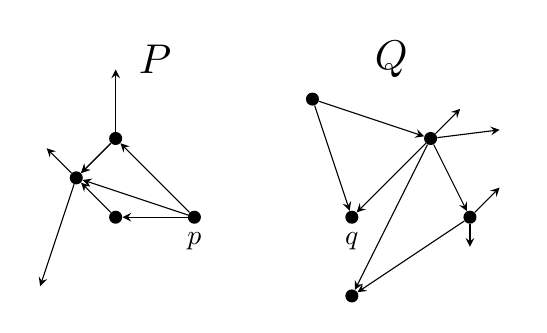
\begin{tikzpicture}
	\node[scale=0.5, circle, fill](p) at (1,0) {};
	\node[scale=0.5, circle, fill](p1) at (0,0) {};
	\node[scale=0.5, circle, fill](p2) at (-.5,.5) {};
	\node[scale=0.5, circle, fill](p3) at (0,1) {};
	\node(p21) at (-1,1) {};
	\node(p22) at (-1,-1) {};
	\node(p31) at (0,2) {};

	\node[scale=0.5, circle, fill](q) at (3,0) {};
	\node[scale=0.5, circle, fill](q1) at (2.5,1.5) {};
	\node[scale=0.5, circle, fill](q2) at (4,1) {};
	\node[scale=0.5, circle, fill](q3) at (3,-1) {};
	\node[scale=0.5, circle, fill](q4) at (4.5,0) {};
	\node(q21) at (4.5,1.5) {};
	\node(q22) at (5,1.125) {};
	\node(q41) at (4.5, -.5) {};
	\node(q42) at (5,.5) {};

	\node at (1,-.3) {$p$};
	\node at (3,-.3) {$q$};

	\draw[->,>=stealth](p) -- (p1);
	\draw[->,>=stealth](p) -- (p3);
	\draw[->,>=stealth](p1) -- (p2);
	\draw[->,>=stealth](p) -- (p2);
	\draw[->,>=stealth](p3) -- (p2);
	\draw[->,>=stealth](p3) -- (p2);
	\draw[->,>=stealth](p2) -- (p21);
	\draw[->,>=stealth](p2) -- (p22);
	\draw[->,>=stealth](p3) -- (p31);

	\draw[->,>=stealth](q1) -- (q);
	\draw[->,>=stealth](q2) -- (q);
	\draw[->,>=stealth](q1) -- (q2);
	\draw[->,>=stealth](q2) -- (q4);
	\draw[->,>=stealth](q2) -- (q3);
	\draw[->,>=stealth](q2) -- (q21);
	\draw[->,>=stealth](q2) -- (q22);
	\draw[->,>=stealth](q4) -- (q3);
	\draw[->,>=stealth](q4) -- (q41);
	\draw[->,>=stealth](q4) -- (q42);

	\node[scale=1.5] at (.5,2) {$P$};
	\node[scale=1.5] at (3.5,2) {$Q$};
\end{tikzpicture}
\\
\vspace{.75cm}
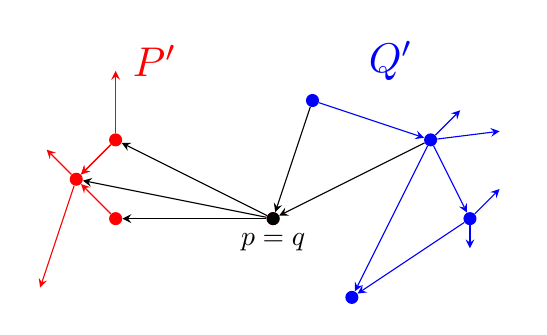
\begin{tikzpicture}
	\node[scale=0.5, circle, fill,color=red](p) at (2,0) {};
	\node[scale=0.5, circle, fill,color=red](p1) at (0,0) {};
	\node[scale=0.5, circle, fill,color=red](p2) at (-.5,.5) {};
	\node[scale=0.5, circle, fill,color=red](p3) at (0,1) {};
	\node(p21) at (-1,1) {};
	\node(p22) at (-1,-1) {};
	\node(p31) at (0,2) {};

	\node[scale=0.5, circle, fill           ](q) at (2,0) {};
	\node[scale=0.5, circle, fill,color=blue](q1) at (2.5,1.5) {};
	\node[scale=0.5, circle, fill,color=blue](q2) at (4,1) {};
	\node[scale=0.5, circle, fill,color=blue](q3) at (3,-1) {};
	\node[scale=0.5, circle, fill,color=blue](q4) at (4.5,0) {};
	\node(q21) at (4.5,1.5) {};
	\node(q22) at (5,1.125) {};
	\node(q41) at (4.5, -.5) {};
	\node(q42) at (5,.5) {};

	\node at (2,-.3) {$p=q$};

	\draw[->,>=stealth](p) -- (p1);
	\draw[->,>=stealth](p) -- (p3);
	\draw[->,>=stealth,color=red](p1) -- (p2);
	\draw[->,>=stealth](p) -- (p2);
	\draw[->,>=stealth,color=red](p3) -- (p2);
	\draw[->,>=stealth,color=red](p3) -- (p2);
	\draw[->,>=stealth,color=red](p2) -- (p21);
	\draw[->,>=stealth,color=red](p2) -- (p22);
	\draw[->,>=stealth,color=red](p3) -- (p31);

	\draw[->,>=stealth](q1) -- (q);
	\draw[->,>=stealth](q2) -- (q);
	\draw[->,>=stealth,color=blue](q1) -- (q2);
	\draw[->,>=stealth,color=blue](q2) -- (q4);
	\draw[->,>=stealth,color=blue](q2) -- (q3);
	\draw[->,>=stealth,color=blue](q2) -- (q21);
	\draw[->,>=stealth,color=blue](q2) -- (q22);
	\draw[->,>=stealth,color=blue](q4) -- (q3);
	\draw[->,>=stealth,color=blue](q4) -- (q41);
	\draw[->,>=stealth,color=blue](q4) -- (q42);

	\node[scale=1.5,color=red] at (.5,2) {$P'$};
	\node[scale=1.5,color=blue] at (3.5,2) {$Q'$};
\end{tikzpicture}
\end{center}

Now, assume that there is indeed a cycle in $S$. 
Note that this cycle must contain the vertex $p=q$, 
(otherwise, we could isolate this cycle in either $P'\subset P$ or 
$Q'\subset Q$ and both of these quivers are, by assumption, acyclic)

Since, however, $p=q$ is the only vertex connecting the two ``lobes'' of $S$, 
this means that the cycle containing $p=q$ can be simplified to a cycle 
contained entirely in $P$ or in $Q$. (BWOC, sps that the cycle contains 
loop components in both $P$ and $Q$. Then since these two quivers are 
disjoint except for $p=q$, then they both must contain $p=q$, and 
the arrows and vertices for each loop component are contained entirely in 
the respective quivers $P, Q$. 
Thus $P$ contains a cycle, as does $Q$. A contradiction)
\end{framed}

Claim: $dim(S)=dim(P)+dim(Q)$. \\
\begin{framed}
Recall: $dim(S)=|S_1|-|S_0|+1$. Now, since this method of gluing 
results in a quiver with all of the arrows from both, and 
all vertices from both with two identified together, we have: 
$$|S_1|=|P_1|+|Q_1|, ~~~ |S_0|=|P_0|+|Q_0|-1$$

Then $$|S_1|-|S_0|+1=\big(|P_1|+|Q_1|\big)-
\big(|P_0|+|Q_0|-1\big)+1$$
Rearranging, we get: 
$$dim(S)=|S_1|-|S_0|+1=\big(|P_1|-|P_0|+1\big)+
\big(|Q_1|-|Q_0|+1\big)=dim(P)+dim(Q)$$
\end{framed}

\section{Gluing arrows}
\textbf{Example} Glue the 1-dimesional quiver \oneDimQ to the 2-dimensional one by identifying an arrow. 
There are 8 possible gluings: $a_1\in\{b_1,...,b_4\}$ and $a_2\in\{b_1,...b_4\}$

For the case $a_1=b_1$, we have then: 
	\tikz[baseline,every node/.style={anchor=base}]{
	\node[scale=.45,circle,draw,inner sep=0pt] (v1) at (0,0){$v_1$};
	\node[scale=.45,circle,draw,inner sep=0pt] (v2) at (1,0){$v_2$};
	\node[scale=.45,circle,draw,inner sep=0pt] (v3) at (2,0){$w_3$};
	\draw[           ->] (v1) to node[scale=.65,midway,above] {$a_1/b_1$} (v2);
	\draw[bend right,->] (v1) to node[scale=.75,midway,below] {$b_2$} (v2);
	\draw[bend left, ->] (v2) to node[scale=.75,midway,above] {$b_3$} (v3);
	\draw[bend right,->] (v2) to node[scale=.75,midway,below] {$b_4$} (v3);
	\draw[bend left, ->] (v1) to [out=80, in=100, looseness=1.5, edge node={node[scale=.75, above]{$a_2$}}] (v2);
	}

Claim: joining 2 acyclic quivers by identifying an arrow from each (following orientation) yields an acyclic quiver. \\
\begin{framed}
Let $P$, $Q$ be two acyclic quivers, and $S$ be the directed graph obtained by 
identifying arrow $a_1\in P$ with arrow $a_2\in Q$. For simplicity, 
we will now call this arrow as simply $a\in S_1\cap P_1\cap Q_1$. 
\begin{center}
	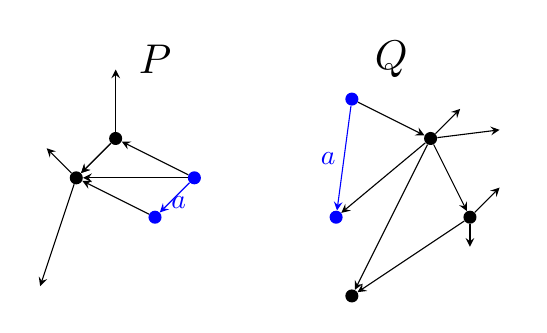
\begin{tikzpicture}
	\node[scale=0.5, circle, fill, color=blue](p) at (1,.5) {};
	\node[scale=0.5, circle, fill, color=blue](p1) at (.5,0) {};
	\node[scale=0.5, circle, fill](p2) at (-.5,.5) {};
	\node[scale=0.5, circle, fill](p3) at (0,1) {};
	\node(p21) at (-1,1) {};
	\node(p22) at (-1,-1) {};
	\node(p31) at (0,2) {};

	\node[scale=0.5, circle, fill, color=blue](q) at (2.8,0) {};
	\node[scale=0.5, circle, fill, color=blue](q1) at (3,1.5) {};
	\node[scale=0.5, circle, fill](q2) at (4,1) {};
	\node[scale=0.5, circle, fill](q3) at (3,-1) {};
	\node[scale=0.5, circle, fill](q4) at (4.5,0) {};
	\node(q21) at (4.5,1.5) {};
	\node(q22) at (5,1.125) {};
	\node(q41) at (4.5, -.5) {};
	\node(q42) at (5,.5) {};

	\draw[->,>=stealth,color=blue](p) to (p1);
	\node[color=blue] at (.8,.18) {$a$};
	\node[color=blue] at (2.7,.75) {$a$};
	\draw[->,>=stealth](p) -- (p3);
	\draw[->,>=stealth](p1) -- (p2);
	\draw[->,>=stealth](p) -- (p2);
	\draw[->,>=stealth](p3) -- (p2);
	\draw[->,>=stealth](p3) -- (p2);
	\draw[->,>=stealth](p2) -- (p21);
	\draw[->,>=stealth](p2) -- (p22);
	\draw[->,>=stealth](p3) -- (p31);

	\draw[->,>=stealth,color=blue](q1) to (q);
	\draw[->,>=stealth](q2) -- (q);
	\draw[->,>=stealth](q1) -- (q2);
	\draw[->,>=stealth](q2) -- (q4);
	\draw[->,>=stealth](q2) -- (q3);
	\draw[->,>=stealth](q2) -- (q21);
	\draw[->,>=stealth](q2) -- (q22);
	\draw[->,>=stealth](q4) -- (q3);
	\draw[->,>=stealth](q4) -- (q41);
	\draw[->,>=stealth](q4) -- (q42);

	\node[scale=1.5] at (.5,2) {$P$};
	\node[scale=1.5] at (3.5,2) {$Q$};
	\end{tikzpicture}\\
\vspace{.75cm}
	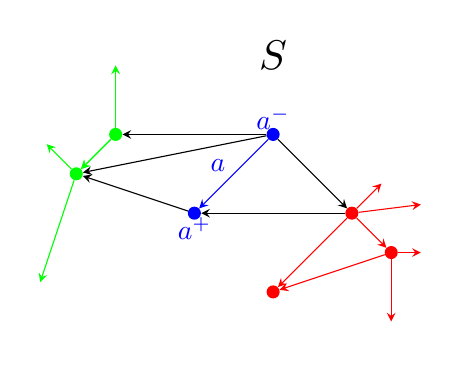
\begin{tikzpicture}
	\node[scale=0.5, circle, fill, color=blue](p) at (2,1) {};\node[color=blue] at (2,1.2) {$a^-$};
	\node[scale=0.5, circle, fill, color=blue](p1) at (1,0) {};\node[color=blue] at (1,-.2) {$a^+$};
	\node[scale=0.5, circle, fill, color=green](p2) at (-.5,.5) {};
	\node[scale=0.5, circle, fill, color=green](p3) at (0,1) {};
	\node(p21) at (-1,1) {};
	\node(p22) at (-1,-1) {};
	\node(p31) at (0,2) {};

	\node[scale=0.5, circle, fill, color=red](q2) at (3,0) {};
	\node[scale=0.5, circle, fill, color=red](q3) at (2,-1) {};
	\node[scale=0.5, circle, fill, color=red](q4) at (3.5,-.5) {};
	\node(q21) at (3.5,0.5) {};
	\node(q22) at (4,0.125) {};
	\node(q41) at (3.5, -1.5) {};
	\node(q42) at (4,-.5) {};

	\draw[->,>=stealth,color=blue](p) to (p1);
	\node[color=blue] at (1.3,.6) {$a$};
	\draw[->,>=stealth](p) -- (p3);
	\draw[->,>=stealth](p1) -- (p2);
	\draw[->,>=stealth](p) -- (p2);
	\draw[->,>=stealth,color=green](p3) -- (p2);
	\draw[->,>=stealth,color=green](p3) -- (p2);
	\draw[->,>=stealth,color=green](p2) -- (p21);
	\draw[->,>=stealth,color=green](p2) -- (p22);
	\draw[->,>=stealth,color=green](p3) -- (p31);

	\draw[->,>=stealth](q2) -- (p1);
	\draw[->,>=stealth](p) -- (q2);
	\draw[->,>=stealth,color=red](q2) -- (q4);
	\draw[->,>=stealth,color=red](q2) -- (q3);
	\draw[->,>=stealth,color=red](q2) -- (q21);
	\draw[->,>=stealth,color=red](q2) -- (q22);
	\draw[->,>=stealth,color=red](q4) -- (q3);
	\draw[->,>=stealth,color=red](q4) -- (q41);
	\draw[->,>=stealth,color=red](q4) -- (q42);

	\node[scale=1.5] at (2,2) {$S$};
	\end{tikzpicture}
\end{center}

Denote by $a^+$ and $a^-$ the head and tail resp of arrow $a$. 

Then if the ordered colletion of arrows 
$C=\{\alpha_1,\alpha_2,...\}$ is a cycle in $S$ with 
vertices $V=\{v_1,....,v_{n-1},v_n=v_1\}$, 
we have the following observation: $$a^\pm\in V.$$ 

Note: if only one of the $a^\pm$ is contained in the cycle, then we are in a 
precisely similar situation as that with identifying a single vertex to glue. 

Alternatively, if neither $a^\pm$ is contained in the cycle, then we could 
write $C\subset S\setminus N_a$ where $N_a$ is the set of all edges 
with endpoints one of $a^{\pm}$. 
Again, the acyclic nature of $P$ and $Q$ make this impossible 
($S\setminus N_a$ is composed of two disjoint quivers, 
one $\subset P$ and one $\subset Q$). 

Therefore $V$ must contain both the head and the tail of the arrow $a$. 

WLOG assume that $C$ contains no loops. 
Now, we can write the ordered vertices in $C$ as: 
$$a^-, p_1,...,p_i,a^+,q_1,...,q_j,a^-$$ where the $p_k\in P$ and $q_k\in Q$. 
(otherwise $C$ would contain a loop). 
Then note that $S$ also contains the cycle 
$$a^-,a^+,q_1,...,q_j,a^-,$$ since $a\in S_1$. 
But note that $a^\pm\subset Q_0$, since $a\in Q_1$. Therefore 
$Q$ contains the cycle given above, a contradiction. 

Therefore $S$ does not contain any cycle. 
\end{framed}

Claim: $dim(S)=dim(P)+dim(Q)$.\\
\begin{framed}
By simple observation, we see that  $$|S_1|=|P_1|+|Q_1|-1$$
and similarly, since the head of each arrow is identified together 
and the tail of each is identified together, $$|S_0|=|P_0|+|Q_0|-2$$
Therefore: 
$$dim(S)=|S_1|-|S_0|+1=
|P_1|+|Q_1|-1-|P_0|-|Q_0|+2+1=\big(|P_1|-|P_0|+1\big)+\big(|Q_1|-|Q_0|+1\big)$$
\end{framed}

\end{document}
